\documentclass[12pt,letterpaper]{article}

% ---------------------- Paquetes ----------------------
\usepackage[spanish,es-tabla]{babel}
\usepackage[utf8]{inputenc}
\usepackage[T1]{fontenc}
\usepackage{geometry}
\usepackage{graphicx}
\usepackage{float}
\usepackage{amsmath, amssymb, siunitx}
\usepackage{hyperref}
\usepackage{setspace}
\usepackage{enumitem}
\usepackage{parskip}
\usepackage{booktabs}
\usepackage{subfig}
\usepackage{multirow}
\usepackage{url}

% ---------------------- Configuración ----------------------
\geometry{margin=1in}
\sisetup{output-decimal-marker={,}}
\onehalfspacing

% ---------------------- Portada ----------------------
\newcommand{\titulo}{Plataforma Web para Apoyo en Procesos de Manufactura}
\newcommand{\universidad}{Pontificia Universidad Javeriana}
\newcommand{\facultad}{Facultad de Ingeniería}
\newcommand{\asignatura}{Procesos de Manufactura Moderna}
\newcommand{\docente}{Martha Manrique}
\newcommand{\autores}{Jacobo Parra\\Miguel Quintero\\Carolhina Real\\Santiago Castro Zuluaga}
\newcommand{\fecha}{Marzo de 2026}

\begin{document}

% ---------------------- Portada ----------------------
\begin{titlepage}
    \centering
    {\huge\bfseries\titulo\par}
    \vspace{1cm}
    {\Large\universidad\\[0.2cm]\facultad\\[0.4cm]\asignatura\par}
    \vspace{0.8cm}
    {\large Docente: \docente\par}
    \vspace{1.2cm}
    {\large\autores\par}
    \vspace{1cm}
    
\includegraphics[width=0.4\textwidth]{javeriana-logo-1.png}
    \vfill
    {\large\fecha\par}
\end{titlepage}

% ---------------------- Introducción ----------------------

\section{Introducción}

En la ingeniería moderna, el acceso eficiente a información técnica constituye un factor clave para el aprendizaje, la documentación de procesos y la difusión del conocimiento científico. En particular, en el área de manufactura, las plataformas digitales permiten presentar conceptos, metodologías y procesos industriales de manera estructurada y accesible.

Las tecnologías web se han convertido en herramientas fundamentales para el desarrollo de recursos educativos interactivos. Mediante el uso de plataformas web, es posible integrar contenido teórico, representaciones visuales, explicaciones técnicas y recursos de apoyo que facilitan la comprensión de procesos de ingeniería.

El presente informe describe el desarrollo y funcionamiento de una plataforma web diseñada para apoyar el aprendizaje de conceptos relacionados con procesos de manufactura. La plataforma se implementa mediante tecnologías web estándar y se encuentra publicada a través de un sistema de alojamiento basado en repositorios de control de versiones, lo cual permite mantener una estructura organizada del proyecto y facilitar la actualización continua del contenido.

El documento presenta la arquitectura general del sistema, la estructura de la plataforma, la lógica de funcionamiento y el flujo de interacción entre los distintos componentes tecnológicos que permiten su operación.

% ---------------------- Objetivos ----------------------

\section{Objetivos}

\subsection{Objetivo general}

Desarrollar y documentar una plataforma web que permita presentar y organizar contenidos relacionados con procesos de manufactura, facilitando el acceso a información técnica y material educativo para estudiantes de ingeniería.

\subsection{Objetivos específicos}

\begin{itemize}

\item Diseñar una plataforma digital que permita presentar información estructurada sobre procesos de manufactura.

\item Implementar una arquitectura basada en tecnologías web estándar que garantice accesibilidad y facilidad de mantenimiento.

\item Utilizar un sistema de control de versiones que permita gestionar el desarrollo del proyecto y su actualización continua.

\item Documentar la estructura lógica y funcional del sistema mediante diagramas de flujo y descripciones técnicas.

\end{itemize}

% ---------------------- Descripción de la plataforma ----------------------

\section{Descripción general de la plataforma}

La plataforma desarrollada corresponde a un sitio web educativo cuyo propósito es presentar información relacionada con conceptos fundamentales de procesos de manufactura.

El sistema está construido utilizando tecnologías web estándar ampliamente utilizadas en el desarrollo de aplicaciones web, entre las cuales se encuentran:

\begin{itemize}

\item \textbf{HTML (HyperText Markup Language):} utilizado para estructurar el contenido de las páginas web y definir la organización de la información.

\item \textbf{CSS (Cascading Style Sheets):} empleado para controlar la presentación visual del sitio, incluyendo estilos, distribución de elementos y diseño de la interfaz.

\item \textbf{JavaScript:} utilizado para proporcionar interactividad dentro de la plataforma y mejorar la experiencia del usuario durante la navegación.

\end{itemize}

La plataforma se encuentra alojada mediante un servicio de publicación de páginas web estáticas que permite desplegar automáticamente el sitio a partir de los archivos almacenados en un repositorio digital. Este tipo de infraestructura permite mantener una arquitectura simple, robusta y de fácil mantenimiento, especialmente adecuada para proyectos educativos y académicos.

% ---------------------- Arquitectura del sistema ----------------------

\section{Arquitectura del sistema}

Desde la perspectiva de ingeniería de software, la plataforma sigue una arquitectura cliente-servidor basada en contenido web estático. Este tipo de arquitectura se caracteriza por separar claramente los componentes responsables del almacenamiento de la información, la publicación del contenido y la interacción con el usuario final.

El sistema se compone de tres elementos principales.

\subsection{Repositorio del proyecto}

El repositorio constituye el núcleo del sistema de desarrollo. En este se almacenan todos los archivos que conforman la plataforma web, incluyendo:

\begin{itemize}

\item Archivos HTML correspondientes a las páginas del sitio.
\item Hojas de estilo CSS utilizadas para el diseño visual.
\item Archivos JavaScript encargados de la lógica interactiva.
\item Recursos gráficos como imágenes y diagramas.

\end{itemize}

El uso de un repositorio permite implementar un sistema de control de versiones, el cual facilita la gestión de cambios, el trabajo colaborativo y la trazabilidad del desarrollo del proyecto.

\subsection{Servidor de publicación}

El servidor de publicación es el componente encargado de desplegar el sitio web en internet. Este sistema toma los archivos almacenados en el repositorio y los convierte en una página web accesible a través de una dirección URL pública.

Cada actualización realizada en el repositorio puede reflejarse automáticamente en la plataforma publicada, lo cual permite mantener el contenido actualizado de manera eficiente.

En este caso la plataforma que elegimos fue GitHub Pages para esta ya que no tiene costo para un trafico web bajo. 

El link en dond se encuentra es este: \\
https://santag207.github.io/manufacturapuj.github.io/

\subsection{Cliente (navegador web)}

El cliente corresponde al usuario final que accede a la plataforma mediante un navegador web. El navegador interpreta los archivos HTML, CSS y JavaScript enviados por el servidor y los transforma en una interfaz gráfica que puede ser visualizada e interactuada por el usuario.

Este proceso permite presentar la información técnica de manera estructurada y comprensible.

% ---------------------- Estructura de la plataforma ----------------------

\section{Estructura de la plataforma}

La plataforma se organiza mediante una estructura jerárquica de páginas que permite presentar la información de manera clara y ordenada.

Entre los componentes principales del sitio se encuentran:

\begin{itemize}

\item Página principal con información introductoria.
\item Secciones dedicadas a diferentes conceptos de manufactura.
\item Recursos visuales y explicativos que apoyan el aprendizaje.
\item Elementos de navegación que permiten desplazarse entre las diferentes secciones del sitio.

\end{itemize}

Esta estructura facilita la consulta de información técnica y permite que los usuarios accedan rápidamente a los contenidos de interés.

% ---------------------- Funcionamiento ----------------------

\section{Lógica de funcionamiento de la plataforma}

El funcionamiento general del sistema sigue una secuencia lógica que describe el proceso mediante el cual un usuario accede a la información publicada.

\begin{enumerate}

\item El usuario accede a la dirección web de la plataforma utilizando un navegador.

\item El navegador envía una solicitud al servidor donde se encuentra alojado el sitio web.

\item El servidor identifica la página solicitada y recupera los archivos correspondientes desde el repositorio del proyecto.

\item Los archivos HTML, CSS y JavaScript son enviados al navegador del usuario.

\item El navegador interpreta estos archivos y renderiza la página web, permitiendo visualizar el contenido y navegar dentro de la plataforma.

\end{enumerate}

Este proceso ocurre de manera casi instantánea y permite que la información técnica sea presentada al usuario de forma clara y organizada.

% ---------------------- Diagrama ----------------------

\section{Diagrama de flujo del sistema}

El siguiente diagrama ilustra el flujo general de funcionamiento de la plataforma web, mostrando la interacción entre el usuario, el navegador, el servidor de publicación y el repositorio del proyecto.

\begin{figure}[H]
\centering
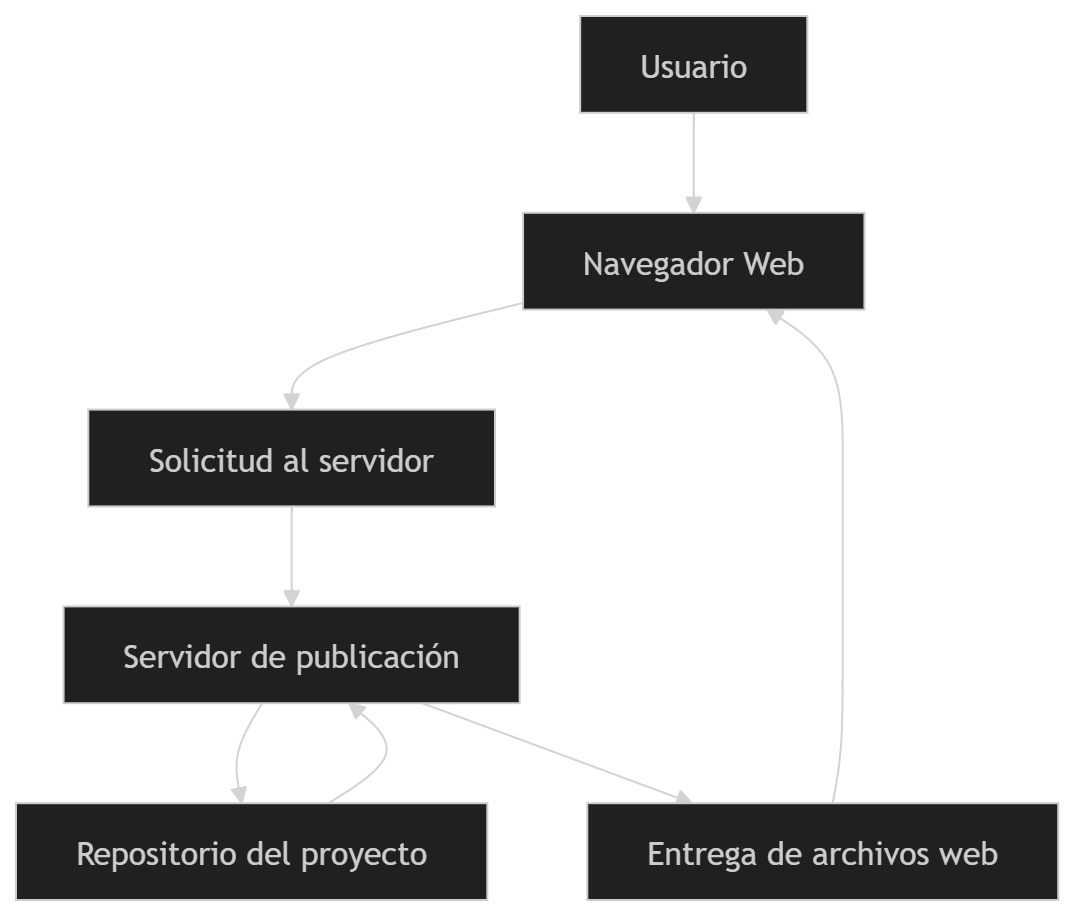
\includegraphics[width=0.8\textwidth]{diagrama_flujo_plataforma.png}
\caption{Diagrama de flujo lógico de funcionamiento de la plataforma web.}
\end{figure}

El diagrama permite visualizar cómo la solicitud del usuario se procesa a través del sistema hasta generar la respuesta final que se presenta en el navegador.

% ---------------------- Aplicación en manufactura ----------------------

\section{Aplicación en el contexto de la manufactura}

En el contexto de la ingeniería de manufactura, el acceso estructurado a información técnica constituye un elemento fundamental para la comprensión de los procesos productivos, la selección adecuada de materiales y el análisis de las distintas metodologías de transformación industrial. En este sentido, las plataformas digitales se han convertido en herramientas de gran importancia para la difusión del conocimiento técnico y la documentación de procesos de fabricación.

La manufactura moderna se caracteriza por integrar conocimientos provenientes de múltiples áreas de la ingeniería, tales como la ciencia de materiales, la mecánica de sólidos, la termodinámica, la ingeniería de procesos y el diseño de productos. Debido a la complejidad de estas disciplinas, resulta necesario contar con herramientas que permitan organizar la información de manera clara, estructurada y fácilmente accesible. Las plataformas web educativas permiten cumplir esta función mediante la integración de contenido técnico, material visual y explicaciones conceptuales dentro de un entorno digital interactivo.

Desde el punto de vista académico, el uso de plataformas digitales facilita el aprendizaje progresivo de los distintos procesos de manufactura, permitiendo que los estudiantes comprendan tanto los principios teóricos como las aplicaciones prácticas que se presentan en la industria. En particular, este tipo de plataformas permite presentar información relacionada con propiedades de materiales, métodos de transformación, parámetros de proceso y criterios de selección de técnicas de fabricación.

Entre los principales beneficios del uso de plataformas digitales para el aprendizaje de procesos de manufactura se encuentran:

\begin{itemize}

\item \textbf{Acceso estructurado a información técnica}: los contenidos pueden organizarse de forma jerárquica, permitiendo que los usuarios consulten conceptos fundamentales, procesos específicos y material complementario de manera ordenada.

\item \textbf{Visualización clara de procesos industriales}: mediante diagramas, esquemas y recursos gráficos es posible representar etapas de producción, flujos de proceso y configuraciones de maquinaria utilizadas en manufactura.

\item \textbf{Facilitación del aprendizaje conceptual}: la integración de explicaciones técnicas con representaciones visuales permite comprender mejor fenómenos asociados a la deformación de materiales, transferencia de calor, solidificación o remoción de material.

\item \textbf{Disponibilidad permanente del material}: al tratarse de una plataforma web, el contenido puede consultarse en cualquier momento y desde diferentes dispositivos, lo cual facilita el estudio autónomo y la revisión de conceptos.

\item \textbf{Actualización continua del contenido}: el uso de sistemas de control de versiones permite mejorar progresivamente el material educativo, incorporar nuevas secciones y corregir información cuando sea necesario.

\end{itemize}

En el ámbito de la ingeniería de manufactura, una plataforma digital como la desarrollada puede utilizarse para documentar y explicar diferentes categorías de procesos productivos utilizados en la industria. Entre los principales procesos que pueden presentarse mediante este tipo de sistemas se encuentran:

\begin{itemize}

\item \textbf{Procesos de mecanizado}: incluyen operaciones de remoción de material como torneado, fresado, taladrado y rectificado. Estos procesos permiten obtener geometrías precisas mediante el uso de herramientas de corte y máquinas herramienta.

\item \textbf{Procesos de manufactura aditiva}: también conocidos como procesos de impresión 3D, consisten en la fabricación de piezas mediante la adición sucesiva de material capa por capa. Estos procesos permiten producir geometrías complejas y son ampliamente utilizados en prototipado rápido.

\item \textbf{Procesos de conformado}: comprenden métodos mediante los cuales un material se deforma plásticamente para adquirir una forma específica sin remover material. Ejemplos de estos procesos incluyen laminado, extrusión, estampado y forjado.

\item \textbf{Procesos de fundición}: consisten en la fabricación de piezas mediante la fusión de un material metálico que posteriormente se vierte en un molde donde solidifica adquiriendo la forma deseada.

\item \textbf{Procesos de moldeo para materiales poliméricos}: utilizados principalmente en la industria de plásticos, incluyen técnicas como moldeo por inyección, moldeo por soplado y termoformado.

\end{itemize}

Además de presentar los procesos de manufactura, las plataformas digitales también pueden utilizarse para explicar aspectos fundamentales relacionados con la ingeniería de materiales, tales como las propiedades mecánicas de los materiales, la microestructura de los metales y polímeros, los tratamientos térmicos y los criterios de selección de materiales en el diseño de productos.

Desde una perspectiva educativa, la integración de estos contenidos dentro de una plataforma web permite mejorar significativamente la comprensión de los procesos industriales, ya que los estudiantes pueden explorar los conceptos a su propio ritmo y complementar las explicaciones teóricas presentadas en clase con material visual y documentación técnica adicional.

Asimismo, este tipo de herramientas digitales contribuye a acercar el entorno académico a las prácticas utilizadas en la industria moderna, donde la digitalización de procesos, la documentación técnica y el uso de sistemas de información forman parte fundamental de la gestión de la manufactura.

En consecuencia, el desarrollo de plataformas web orientadas a la documentación de procesos de manufactura representa una estrategia valiosa para fortalecer la formación de ingenieros, permitiendo integrar conocimientos teóricos, recursos visuales y herramientas digitales dentro de un mismo entorno educativo.

% ---------------------- Conclusiones ----------------------

\section{Conclusiones}

El desarrollo de la plataforma web permitió implementar una herramienta digital orientada a la organización y difusión de contenidos relacionados con procesos de manufactura. A través de una estructura clara y accesible, el sistema facilita la consulta de información técnica y contribuye a mejorar la comprensión de distintos conceptos asociados a la ingeniería de manufactura.

Desde el punto de vista tecnológico, la implementación de la plataforma mediante tecnologías web estándar como HTML, CSS y JavaScript permitió construir un sistema ligero, eficiente y fácilmente mantenible. Este enfoque basado en páginas web estáticas reduce la complejidad de la infraestructura requerida y permite que el sitio pueda ser desplegado de manera sencilla utilizando servicios de alojamiento especializados en este tipo de aplicaciones.

El uso de un repositorio con control de versiones representa además una ventaja significativa en el desarrollo del proyecto, ya que permite mantener un registro estructurado de las modificaciones realizadas, facilitar el trabajo colaborativo entre los integrantes del equipo y garantizar la trazabilidad de las diferentes versiones del sistema. Esta metodología de desarrollo es ampliamente utilizada en proyectos tecnológicos y resulta especialmente útil en entornos académicos donde múltiples usuarios participan en la construcción del contenido.

Desde una perspectiva educativa, la plataforma desarrollada demuestra el potencial de las herramientas digitales para apoyar el aprendizaje en áreas de ingeniería. La organización estructurada de la información, junto con la posibilidad de integrar recursos visuales y explicaciones técnicas, permite complementar los procesos de enseñanza tradicionales y facilitar la comprensión de conceptos asociados a procesos industriales y de manufactura.

Complementariamente, este tipo de iniciativas contribuye a fortalecer la integración entre herramientas tecnológicas y formación en ingeniería, promoviendo el uso de plataformas digitales como medios efectivos para la difusión de conocimiento técnico y la documentación de procesos de manufactura dentro del entorno académico.

\end{document}